\section{IP address allocation dynamics}
\label{sec:allocations}

In this section we present an evaluation of IP block allocations. We examine 
allocation block sizes over time, as well as a yearly distribution of IP 
allocations. We also measured the IP block allocation dynamics geographically,
to see differences across different nations.

\subsection{Allocated IP block sizes}

The data show a number of highlights about allocated block sizes over the past
six years. Figure \ref{fig:IP allocations} illustrates several changes that
are observable. It shows the number of allocations increasing for every prefix
length in every year, though at different rates. In all years, clearly /24
prefix allocations are the most prevalent. Interestingly, in 2003 there were
only about half as many /20 allocations as /19 ones, whereas in 2008 they were
about at parity. Thus the smaller allocation blocks grew in number at a rate
higher than the shorter /19 prefixes. At the same time, noticeably there has
been almost no increase in /16 blocks. Overall, this shows the growing trend
toward smaller blocks as the IPv4 address space approaches saturation. In
summary, most IP allocations over the six-year period are /24 blocks. The next
most popular block size is /16, followed by /19 and /20. Finally, smaller
block sizes (/19 and smaller) have had a larger increase in usage than /16,
/17, and /18.

\begin{figure}[htbp]
 	\centering
 		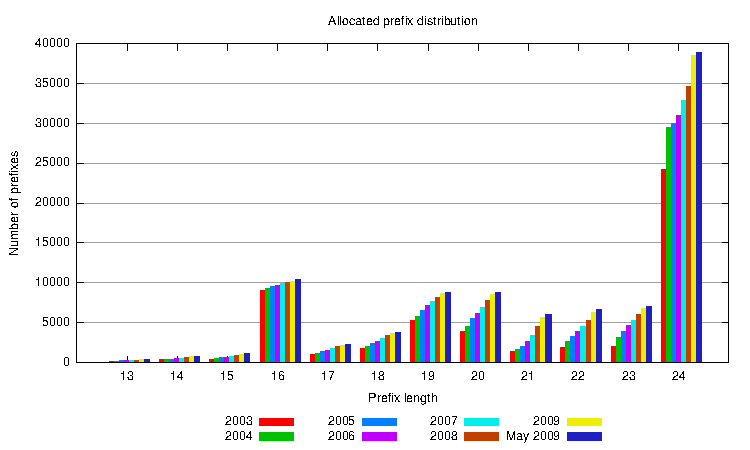
\includegraphics[width=0.5\textwidth]{02_prefixes/02_ip_prefixes_zoom}
	\caption{Allocated prefix distribution}
 	\label{fig:IP allocations}
\end{figure}

\subsection{Yearly distribution of IP allocations}

% \begin{figure}[htbp]
%  	\centering
%  		 \includegraphics[width=0.5\textwidth]{04_plus_minus/addremoveprefixallocculmulative}
% 	\caption{Trends in IP prefix allocation}
%  	\label{fig:IP allocations new and gone}
% \end{figure}

Aggregated together, the number of new allocations over the time period
studied is over 40,000. Figure \ref{fig:IP allocations new and gone} charts
the occurrence of other events that factor into the net allocation count
increase. These include prefix splitting, prefix extension, and deallocation.
Prefix splitting is the dividing of one prefix into multiple smaller prefixes.
Prefix extension is the aggregating of an existing prefix with its adjacent,
previously unallocated address space (e.g. a /16 prefix might become a /15
prefix by including the adjacent /16 address space). Deallocation is the
withdrawing of a prefix allocation, essentially releasing IP space for later
use. Figure \ref{fig:IP allocations new and gone}, charts these factors that
increase the count of allocations. Some of the increase is attributable to new
allocations. A smaller amount was due to prefix splitting. A small decrease in
the allocations count resulted from prefix extension. Finally, a larger
decrease was due to deallocation, although the number of new allocations has
greatly outpaced the disappearances.

\begin{figure}[htbp]
    \centering
        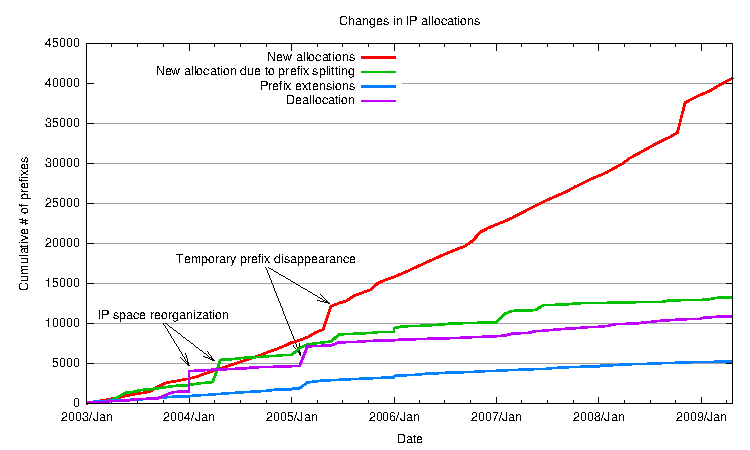
\includegraphics[width=\columnwidth]{04_3_plus_minus/changes}
    \caption{Changes in IP allocations}
    \label{fig:IP allocations new and gone}
\end{figure}

There is one illustration that particularly shows the dynamic character of IP
allocation records. Figure \ref{fig:alloc ages total} plots the number of
prefixes allocated each year, according to snapshots taken in the years from
2003 to 2009 (shown in different colors). It is interesting to note that in
more recent years, the record of prefixes allocated during the 1990s has
increased. This increase is especially prominent in the past year. Among other
reasons, this is indicative of prefix splitting, where a larger allocated
block is split into multiple blocks. When blocks are split, the resulting
blocks retain the year of origin of the block under which they were originally
allocated. Figure \ref{fig:alloc ages total} shows that while many of the
existing allocations originated in the 90s, many of these also are blocks
split off larger ones that were allocated at the time.

\begin{figure}[htbp]
	\centering
		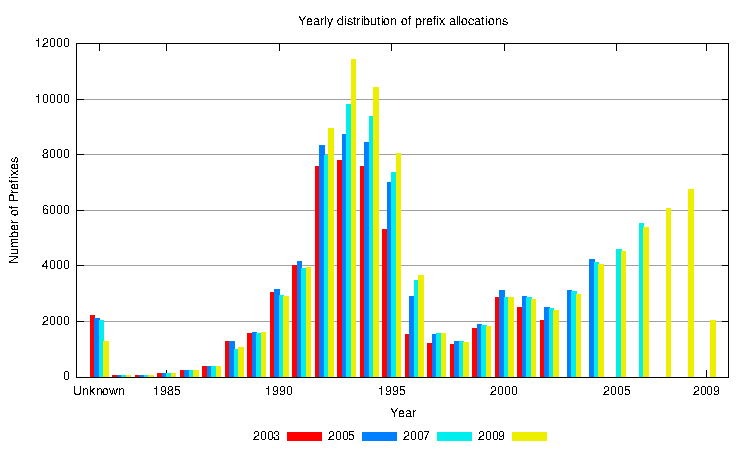
\includegraphics[width=\columnwidth]{10_alloc_ages/alloc_total}
	\caption{Records of IP allocations, from the perspective the given years
		     2003--2009 (odd-numbered years shown only, for clarity)}
	% \newline
	% * Note that in successive years, the known number of allocations recorded tends
	% to rise (odd-numbered years shown only, for clarity)}
	\label{fig:alloc ages total}
\end{figure}


\subsection{Unaligned allocation}

There is an occurrence among IP allocations that--while rare--warrants some
attention. Unaligned IP blocks are any allocations of a size that is not some
power of 2. For instance, an unaligned block of 12,288 addresses has been
recently allocated by ARIN (allocation of the block 67.23.0.0-67.23.47.255 on
January 23, 2009). This allocation cannot be represented as a single entry in
the BGP routing table and requires at least a /19 and /20 prefix to express it.
The number of unaligned allocations is very small because they clearly are
wasteful of BGP table space and have insignificant advantages over aligned
ones, if any. Figure~\ref{fig:unaligned IP allocations} shows the distribution
of such allocations. Most were between 1992 and 1995, although a few continue
to be allocated every year since then. Obviously, compared to the size of the
routing table ($>$300K entries) these allocations are negligible in number.
Nonetheless it is interesting to note their continued existence.

\begin{figure}[htbp]
 	\centering
 		\includegraphics[width=0.5\textwidth]{09_alloc_adhoc/adhoc}
	\caption{Unaligned IP allocations per year}
 	\label{fig:unaligned IP allocations}
\end{figure}

\subsection{Allocation by geographical region}

\begin{table*}[p]
%%%%%%%%%%%%%%%%%%%%%%%%%%%%%%%%%%%%%%%%%%%%%%%%%%%%%%%%%%%%%%%%%%%%%%%%%%%%%%%%
%% TOP announced prefixes
%%%%%%%%%%%%%%%%%%%%%%%%%%%%%%%%%%%%%%%%%%%%%%%%%%%%%%%%%%%%%%%%%%%%%%%%%%%%%%%%
\begin{minipage}[t]{0.48\textwidth}
% \begin{table}[p]
	\begin{center}
	\caption{Top 25 countries with the most number of allocated IP blocks on \textbf{January 1, 2003}}
	\label{tab:top25 rir prefixes 2003}
	\begin{tabular}{|l||l|r|r|}
		\hline
		&      \bf Country		& \bf Prefixes  &  \bf  IP space 		\tabularnewline \hline
1       &       US      		&       31,699  &       1,240,486,995   \tabularnewline
2       &       Canada  		&       5,314   &       61,593,600      \tabularnewline
3       &       Germany 		&       1,642   &       49,413,120      \tabularnewline
4       &       UK      		&       1,573   &       74,358,784      \tabularnewline
5       &       Australia       &       1,351   &       22,956,032      \tabularnewline
6       &       Italy   		&       836     &       14,270,464      \tabularnewline
7       &       Switzerland     &       737     &       10,523,904      \tabularnewline
8       &       Japan   		&       674     &       95,166,320      \tabularnewline
9       &       France  		&       625     &       37,038,080      \tabularnewline
10      &       Netherlands     &       619     &       28,387,328      \tabularnewline
11      &       Sweden  		&       533     &       13,377,024      \tabularnewline
12      &       Russia  		&       501     &       6,259,200       \tabularnewline
13      &       Hong Kong       &       491     &       4,476,416       \tabularnewline
14      &       China   		&       393     &       29,396,736      \tabularnewline
15      &       New Zealand     &       366     &       3,820,288       \tabularnewline
16      &       Finland 		&       348     &       8,085,760       \tabularnewline
17      &       Norway  		&       322     &       8,610,304       \tabularnewline
18      &       Spain   		&       310     &       9,625,344       \tabularnewline
19      &       South Africa    &       275     &       8,163,328       \tabularnewline
20      &       Austria 		&       267     &       5,279,232       \tabularnewline
21      &       Brazil  		&       260     &       10,902,784      \tabularnewline
22      &       Chile   		&       251     &       2,310,656       \tabularnewline
23      &       Singapore       &       250     &       1,933,856       \tabularnewline
24      &       Thailand        &       245     &       1,667,328       \tabularnewline
25      &       India   		&       240     &       2,636,032       \tabularnewline
% 26      &       South Korea     &       197     &       26,208,768      \tabularnewline
% 27      &       Indonesia       &       188     &       1,005,568       \tabularnewline
% 28      &       Taiwan  		&       184     &       11,659,008      \tabularnewline
% 29      &       Poland  		&       174     &       3,982,080       \tabularnewline
% 30      &       Belgium 		&       163     &       4,664,832       \tabularnewline
	\hline
	\end{tabular}
	\end{center}
% \end{table}
\end{minipage}
%
\quad
%
\begin{minipage}[t]{0.48\textwidth}
% \begin{table}[p]
	\begin{center}
	\caption{Top 25 countries with the most number of allocated IP blocks on \textbf{April 23, 2009}}
	\label{tab:top25 rir prefixes 2009}
	\begin{tabular}{|l||l|r|r|r|}
		\hline
		&      \bf Country		& \bf Prefixes  &       \bf IP space 	& \bf Change$^{*}$ 	\tabularnewline \hline 
1       &       US      &       36,881  &       1,473,990,144   &         1.16  \tabularnewline
2       &       Australia       &       6,099   &       37,378,304      &         4.51  \tabularnewline
3       &       Canada  &       5,709   &       75,905,792      &         1.07  \tabularnewline
4       &       Germany &       5,612   &       85,205,400      &         3.42  \tabularnewline
5       &       European Union  &       5,074   &       114,168,224     &        46.98  \tabularnewline
6       &       UK      &       3,732   &       70,756,184      &         2.37  \tabularnewline
7       &       Russia  &       3,148   &       24,607,688      &         6.28  \tabularnewline
8       &       Japan   &       2,068   &       153,285,376     &         3.07  \tabularnewline
9       &       France  &       1,814   &       68,384,704      &         2.90  \tabularnewline
10      &       Ukraine &       1,769   &       5,516,480       &        19.88  \tabularnewline
11      &       Poland  &       1,602   &       13,869,704      &         9.21  \tabularnewline
12      &       China   &       1,566   &       191,643,392     &         3.98  \tabularnewline
13      &       Netherlands     &       1,449   &       21,291,560      &         2.34  \tabularnewline
14      &       Switzerland     &       1,359   &       8,249,320       &         1.84  \tabularnewline
15      &       New Zealand     &       1,217   &       6,116,096       &         3.33  \tabularnewline
16      &       Italy   &       955     &       32,206,272      &         1.14  \tabularnewline
17      &       South Africa    &       886     &       15,057,920      &         3.22  \tabularnewline
18      &       Sweden  &       862     &       18,986,400      &         1.62  \tabularnewline
19      &       Austria &       854     &       7,292,128       &         3.20  \tabularnewline
20      &       Romania &       769     &       8,643,328       &        21.36  \tabularnewline
21      &       Czech Republic  &       706     &       6,059,392       &         5.98  \tabularnewline
22      &       South Korea     &       700     &       72,193,792      &         3.55  \tabularnewline
23      &       Finland &       655     &       8,932,864       &         1.88  \tabularnewline
24      &       Hong Kong       &       651     &       8,208,128       &         1.33  \tabularnewline
25      &       India   &       611     &       18,290,432      &         2.55  \tabularnewline
% 26      &       Spain   &       530     &       21,794,976      &         1.71  \tabularnewline
% 27      &       Denmark &       491     &       9,289,824       &         3.43  \tabularnewline
% 28      &       Indonesia       &       482     &       7,263,488       &         2.56  \tabularnewline
% 29      &       Taiwan  &       422     &       24,680,704      &         2.29  \tabularnewline
% 30      &       Argentina       &       421     &       7,395,072       &         2.75  \tabularnewline
	\hline
	\end{tabular}
	\end{center}

	\small	$^{*}$ -- Relative change in number of allocated IP blocks from January 1, 2003 and April 23, 2009
% \end{table}
\end{minipage}

\vspace{1cm}

%%%%%%%%%%%%%%%%%%%%%%%%%%%%%%%%%%%%%%%%%%%%%%%%%%%%%%%%%%%%%%%%%%%%%%%%%%%%%%%%
%% TOP announced IP space
%%%%%%%%%%%%%%%%%%%%%%%%%%%%%%%%%%%%%%%%%%%%%%%%%%%%%%%%%%%%%%%%%%%%%%%%%%%%%%%%
\begin{minipage}[t]{0.48\textwidth}
% \begin{table}[p]
	\begin{center}
	\caption{Top 25 countries with the most allocated IP space on \textbf{January 1, 2003}}
	\label{tab:top25 rir ip space 2003}
	\begin{tabular}{|l||l|r|r|}
		\hline
		&      \bf Country		& \bf Prefixes  &  \bf IP space 		\tabularnewline \hline 
1       &       US      		&       31,699  &       1,240,486,995   \tabularnewline
2       &       Japan   		&       674     &       95,166,320      \tabularnewline
3       &       UK      		&       1,573   &       74,358,784      \tabularnewline
4       &       Canada  		&       5,314   &       61,593,600      \tabularnewline
5       &       Germany 		&       1,642   &       49,413,120      \tabularnewline
6       &       France  		&       625     &       37,038,080      \tabularnewline
7       &       China   		&       393     &       29,396,736      \tabularnewline
8       &       Netherlands     &       619     &       28,387,328      \tabularnewline
9       &       South Korea     &       197     &       26,208,768      \tabularnewline
10      &       Australia       &       1,351   &       22,956,032      \tabularnewline
11      &       Italy   		&       836     &       14,270,464      \tabularnewline
12      &       Sweden  		&       533     &       13,377,024      \tabularnewline
13      &       Taiwan  		&       184     &       11,659,008      \tabularnewline
14      &       Brazil  		&       260     &       10,902,784      \tabularnewline
15      &       Switzerland     &       737     &       10,523,904      \tabularnewline
16      &       Spain   		&       310     &       9,625,344       \tabularnewline
17      &       Norway  		&       322     &       8,610,304       \tabularnewline
18      &       South Africa    &       275     &       8,163,328       \tabularnewline
19      &       Finland 		&       348     &       8,085,760       \tabularnewline
20      &       Russia  		&       501     &       6,259,200       \tabularnewline
21      &       Mexico  		&       132     &       5,644,288       \tabularnewline
22      &       Austria 		&       267     &       5,279,232       \tabularnewline
23      &       Belgium 		&       163     &       4,664,832       \tabularnewline
24      &       Denmark 		&       143     &       4,634,624       \tabularnewline
25      &       Hong Kong       &       491     &       4,476,416       \tabularnewline
% 26      &       Poland  		&       174     &       3,982,080       \tabularnewline
% 27      &       New Zealand     &       366     &       3,820,288       \tabularnewline
% 28      &       European Union  &       108     &       3,149,824       \tabularnewline
% 29      &       India  			&       240     &       2,636,032       \tabularnewline
% 30      &       Israel 			&       81      &       2,579,712       \tabularnewline
	\hline
	\end{tabular}
	\end{center}
	\ \newline\ \newline
% \end{table}
\end{minipage}
%
\quad
%
\begin{minipage}[t]{0.48\textwidth}
% \begin{table}[p]
	\begin{center}
	\caption{Top 25 countries with the most allocated IP space on \textbf{April 23, 2009}}
	\label{tab:top25 rir ip space 2009}
	\begin{tabular}{|l||l|r|r|r|}
		\hline
		&      \bf Country		& \bf Prefixes  &       \bf IP space 	& \bf Change$^{*}$ 	\tabularnewline \hline 
1       &       US      &       36,881  &       1,473,990,144   &         1.19  \tabularnewline
2       &       China   &       1,566   &       191,643,392     &         6.52  \tabularnewline
3       &       Japan   &       2,068   &       153,285,376     &         1.61  \tabularnewline
4       &       European Union  &       5,074   &       114,168,224     &        36.25  \tabularnewline
5       &       Germany &       5,612   &       85,205,400      &         1.72  \tabularnewline
6       &       Canada  &       5,709   &       75,905,792      &         1.23  \tabularnewline
7       &       South Korea     &       700     &       72,193,792      &         2.75  \tabularnewline
8       &       UK      &       3,732   &       70,756,184      &          .95  \tabularnewline
9       &       France  &       1,814   &       68,384,704      &         1.85  \tabularnewline
10      &       Australia       &       6,099   &       37,378,304      &         1.63  \tabularnewline
11      &       Italy   &       955     &       32,206,272      &         2.26  \tabularnewline
12      &       Brazil  &       267     &       29,754,880      &         2.73  \tabularnewline
13      &       Taiwan  &       422     &       24,680,704      &         2.12  \tabularnewline
14      &       Russia  &       3,148   &       24,607,688      &         3.93  \tabularnewline
15      &       Spain   &       530     &       21,794,976      &         2.26  \tabularnewline
16      &       Mexico  &       156     &       21,503,232      &         3.81  \tabularnewline
17      &       Netherlands     &       1,449   &       21,291,560      &          .75  \tabularnewline
18      &       Sweden  &       862     &       18,986,400      &         1.42  \tabularnewline
19      &       India   &       611     &       18,290,432      &         6.94  \tabularnewline
20      &       South Africa    &       886     &       15,057,920      &         1.84  \tabularnewline
21      &       Poland  &       1,602   &       13,869,704      &         3.48  \tabularnewline
22      &       Turkey  &       283     &       10,515,904      &         4.22  \tabularnewline
23      &       Denmark &       491     &       9,289,824       &         2.00  \tabularnewline
24      &       Finland &       655     &       8,932,864       &         1.10  \tabularnewline
25      &       Romania &       769     &       8,643,328       &        12.95  \tabularnewline
% 26      &       Switzerland     &       1,359   &       8,249,320       &          .78  \tabularnewline
% 27      &       Hong Kong       &       651     &       8,208,128       &         1.83  \tabularnewline
% 28      &       Norway  &       419     &       7,425,584       &          .86  \tabularnewline
% 29      &       Argentina       &       421     &       7,395,072       &         3.87  \tabularnewline
% 30      &       Austria &       854     &       7,292,128       &         1.38  \tabularnewline
	\hline
	\end{tabular}
	\end{center}
	\small	$^{*}$ -- Relative change in allocated IP space from January 1, 2003 and April 23, 2009
% \end{table}
\end{minipage}

\end{table*}

% \clearpage

\begin{figure*}[tp]
\begin{minipage}[b]{\textwidth}
\centering

%%%%%%%%%%%%%%%%%%%%%%%%%%%%%%%%%%%%%%%%%%%%%%%%%%%%%%%%%%%%%%%%%%
%% BGP counts
%%%%%%%%%%%%%%%%%%%%%%%%%%%%%%%%%%%%%%%%%%%%%%%%%%%%%%%%%%%%%%%%%%
\begin{minipage}[b]{0.48\textwidth}
% \begin{figure}[p]
	\centering
		\includegraphics[trim=0 17px 0px 76px,clip=true,width=\columnwidth]{00_maps/ip_count_2003}%
		\hspace{-0.98\columnwidth}%
		\includegraphics[width=1cm]{scale_ip_count}\hspace{-1cm}%
		\hspace{0.98\columnwidth}
	\caption{Geographical distribution of number of allocated IP blocks on \textbf{January 1, 2003}}
	\label{fig:rir prefixes 2003}
% \end{figure}
\end{minipage}%
%
\quad
%
\begin{minipage}[b]{0.48\textwidth}
% \begin{figure}[p]
	\centering
		\includegraphics[trim=0 17px 0px 76px,clip=true,width=\columnwidth]{00_maps/ip_count_2009_2}%
		\hspace{-0.98\columnwidth}%
		\includegraphics[width=1cm]{scale_ip_count}\hspace{-1cm}%
		\hspace{0.98\columnwidth}
	\caption{Geographical distribution of number of allocated IP blocks on \textbf{April 23, 2009}}
	\label{fig:rir prefixes 2009}
% \end{figure}
\end{minipage}

\vspace{0.5cm}

%%%%%%%%%%%%%%%%%%%%%%%%%%%%%%%%%%%%%%%%%%%%%%%%%%%%%%%%%%%%%%%%%%
%% BGP sizes
%%%%%%%%%%%%%%%%%%%%%%%%%%%%%%%%%%%%%%%%%%%%%%%%%%%%%%%%%%%%%%%%%%
\begin{minipage}[b]{0.48\textwidth}
% \begin{figure}[p]
	\centering
		\includegraphics[trim=0 17px 0px 76px,clip=true,width=\columnwidth]{00_maps/ip_size_2003}%
		\hspace{-0.98\columnwidth}%
		\includegraphics[width=1cm]{scale_ip_size}\hspace{-1cm}%
		\hspace{0.98\columnwidth}
	\caption{Geographical distribution of allocated IP space on \textbf{January 1, 2003}}
	\label{fig:rir ip space 2003}
% \end{figure}
\end{minipage}%
%
\quad
%
\begin{minipage}[b]{0.48\textwidth}
% \begin{figure}[p]
	\centering
		\includegraphics[trim=0 17px 0px 76px,clip=true,width=\columnwidth]{00_maps/ip_size_2009_2}%
		\hspace{-0.98\columnwidth}%
		\includegraphics[width=1cm]{scale_ip_size}\hspace{-1cm}%
		\hspace{0.98\columnwidth}
	\caption{Geographical distribution of allocated IP space on \textbf{April 23, 2009}}
	\label{fig:rir ip space 2009}
% \end{figure}
\end{minipage}

\vspace{0.5cm}

%%%%%%%%%%%%%%%%%%%%%%%%%%%%%%%%%%%%%%%%%%%%%%%%%%%%%%%%%%%%%%%%%%
%% Asia region
%%%%%%%%%%%%%%%%%%%%%%%%%%%%%%%%%%%%%%%%%%%%%%%%%%%%%%%%%%%%%%%%%%
\begin{minipage}[b]{0.48\textwidth}
% \begin{figure}[p]
	\centering
		\includegraphics[trim=0 17px 0px 76px,clip=true,width=\columnwidth]{00_maps/ip_asia_2009_prefixes}%
		\hspace{-0.98\columnwidth}%
		\includegraphics[width=1cm]{scale_ip_count}\hspace{-1cm}%
		\hspace{0.98\columnwidth}
	\caption{Geographical distribution of number of allocated IP blocks in Asian region on \textbf{April 23, 2009}}
	\label{fig:rir prefixes asia 2009}
% \end{figure}
\end{minipage}%
%
\quad
%
\begin{minipage}[b]{0.48\textwidth}
% \begin{figure}[p]
	\centering
		\includegraphics[trim=0 17px 0px 76px,clip=true,width=\columnwidth]{00_maps/ip_asia_2009_space}%
		\hspace{-0.98\columnwidth}%
		\includegraphics[width=1cm]{scale_ip_size}\hspace{-1cm}%
		\hspace{0.98\columnwidth}
	\caption{Geographical distribution of allocated IP space in Asian region on \textbf{April 23, 2009}}
	\label{fig:rir ip space asia 2009}
% \end{figure}
\end{minipage}

\end{minipage}
\end{figure*}

% \clearpage


In this part we present a number of findings of IP allocations from a 
geographical viewpoint, that is, on a country-based level. The analysis of 
snapshots of IP allocations at fixed times shows which countries are 
allocated more prefixes and gives an understanding of the Internet penetration 
throughout the world.

Table~\ref{tab:top25 rir prefixes 2003} is a list of the 25 countries that 
were allocated the most prefixes in 2003.  With each country is shown what 
size of IP address space is covered by the sets of allocated IP blocks.
Table~\ref{tab:top25 rir ip space 2003} gives an alternative representation, 
re-ordered by descending IP-allocated space.  We note that, for example, 
in 2003 Japan with only 674 allocated prefixes (8th in 
Table~\ref{tab:top25 rir prefixes 2003}) covered more IP (2nd in 
Table~\ref{tab:top25 rir ip space 2003}) space than all other countries 
excluding the United States.  This indicates Japan's allocations efficiently 
cover their IP space.

Tables~\ref{tab:top25 rir prefixes 2009} and ~\ref{tab:top25 rir ip space
2009} present a current estimates for 2009 of the same data, name the 
top 25 contributors to the global routing table and top 25 countries with 
the most announced address space. A comparison of the 2003 and 2009 tables 
shows a marked re-ordering of some countries relative to others, in terms 
of the number of allocations as well as in terms of the number of allocated 
IP addresses. For example, Canada (2nd in 
Table~\ref{tab:top25 rir prefixes 2003}) had relatively small growth over 
the 6 years and is now tied in rank with other regions that made great strides, 
such as Australia (5th in Table~\ref{tab:top25 rir prefixes 2003}, 
2nd in Table~\ref{tab:top25 rir prefixes 2009}) and the European countries 
(a combined entity recognized during the 6-year interval).

Figures~\ref{fig:rir prefixes 2003}--\ref{fig:rir ip space asia 2009} show the
annual number of allocations by colors on a map of the world. The figure pairs 
\ref{fig:rir prefixes 2003} \& \ref{fig:rir prefixes 2009}, and 
\ref{fig:rir ip space 2003} \& \ref{fig:rir ip space 2009}, trace regional Internet 
growth dynamics from a global view.  These world maps repeat the information given 
in Tables~\ref{tab:top25 rir prefixes 2003}--~\ref{tab:top25 rir ip space
2009} but also include relative allocation activity levels for all countries of 
the world.  Figure~\ref{fig:rir prefixes asia 2009} and 
Figure~\ref{fig:rir ip space asia 2009} reiterate the measure of IP space usage
``efficiency'' in one section of the world undergoing tremendous Internet penetration 
and growth.  In East Asia several countries such as Japan and China, using fewer allocated 
block (lighter colors in Figure ~\ref{fig:rir prefixes asia 2009}), 
cover much more IP space (darker colors in Figure~\ref{fig:rir ip space asia 2009}), 
in comparison to a country such as India.

